\documentclass[journal]{IEEEtran}
\usepackage[T1]{fontenc}
\usepackage[utf8]{inputenc}
\usepackage{booktabs,tabularx,array,multirow}
\usepackage{amsmath}
\usepackage{graphicx}
\usepackage{url}
\makeatletter\g@addto@macro\UrlBreaks{\do\_\do\-}\makeatother
\usepackage[hidelinks]{hyperref}
\newcolumntype{L}{>{\raggedright\arraybackslash}X}
\newcommand{\m}{$-$}

\begin{document}

\title{What Do Wrist-Worn Stress Detectors Detect? A Matched-Arousal Specificity Test Across Five Empatica E4 Datasets}

\author{Alvaro~Octavio~Ibarra~Reyes and Chen~Pan%
\thanks{The authors are with the Department of Electrical and Computer Engineering, The University of Texas at San Antonio, San Antonio, TX 78249 USA (e-mail: [email]@utsa.edu; [email]@utsa.edu).}}

\markboth{IEEE Journal of Biomedical and Health Informatics}{Ibarra Reyes and Pan: What Do Wrist-Worn Stress Detectors Detect?}

\maketitle

\begin{abstract}
Wrist-worn stress detectors are trained to separate stressor periods from rest and are reported as detecting stress. It has been suggested that they detect arousal instead. We test this against non-stress arousal states. On five public Empatica E4 datasets with audited labels, a heart-rate, heart-rate-variability and electrodermal model trained on four datasets loses only 0.015--0.05 balanced accuracy on the fifth, and an untrained index of heart rate and tonic electrodermal activity ranks stress as well as the trained model on every dataset. Adding a state to the training negatives removes exercise false alarms (69\% to 8--10\%) but not those on speech and arithmetic without evaluation (55\%), hyperventilation (about 50\%) or manual tasks (43\% to 33\%). At matched heart rate and electrodermal activity the detector cannot separate stress from these states or from anger clips (within-bin AUROC 0.36--0.58, none significant after Holm correction), but separates it from exercise (0.89); what it adds to arousal is shared by every active task. Minutes since recording start predict stress better than physiology on two datasets whose baselines coincide with sensor warm-up. Recovery, sensor loss and onset latency explain at most 0.06 of the 0.22--0.29 within-dataset error, and each subject's own arousal response predicts detection ($\rho=0.56$). Wrist detectors transfer because they detect autonomic arousal, not evaluative stress. We propose a specificity panel and a matched-arousal test as reporting standards and release the label-audit, split and analysis code.
\end{abstract}

\begin{IEEEkeywords}
Wearable stress detection, Empatica E4, autonomic arousal, cross-dataset generalization, specificity, electrodermal activity.
\end{IEEEkeywords}

\section{Introduction}
\IEEEPARstart{S}{tress} detection from wrist wearables is usually posed as classification: windows recorded during a laboratory stressor are labelled stress, windows from rest or a control task non-stress. Reported accuracies are high, and the models are described as detecting stress. Yet the wrist device measures pulse rate, a weak vagal proxy, electrodermal activity (EDA), skin temperature and movement; none of these is stress, and all respond to autonomic arousal from any cause. Zhou et al.~\cite{zhou2023} found that chest-ECG and EDA models trained on a stress corpus transfer to arousal ratings of emotion videos, and concluded that such models ``may be identifying emotional arousal instead of stress''. Kwon et al.~\cite{kwon2026} matched heart rate within subjects and found that the WESAD stress-versus-rest signal survives in EDA and temperature. Neither asked whether a wrist detector separates stress from other arousing non-stress states once cardiac and electrodermal arousal are both matched, which is the test a deployed detector has to pass. The cross-dataset literature also disagrees on whether such detectors transfer at all~\cite{prajod2024,calzametre2026,xiao2025,mishra2020,kwon2026}.

We address both questions on five public E4 datasets whose labels we audited against their descriptor papers. The contributions are:
(1) a specificity test that extends heart-rate matching from rest to non-stress arousal states: at matched heart rate and tonic EDA, a fixed detector separates stress from rest, consistent with Kwon et al., but not from the same speech and arithmetic without evaluation, hyperventilation, manual tasks or anger clips, even when those states are in training; only exercise becomes separable;
(2) a five-dataset leave-one-dataset-out evaluation in which transfer costs 0.015--0.05 balanced accuracy and in which an untrained two-feature arousal index matches the trained model;
(3) protocol position measured as a confound: minutes since recording start out-predict physiology within two datasets because their baselines coincide with sensor warm-up;
(4) a bounded error budget and a dose--response test locating the within-dataset ceiling mainly in the size of each subject's arousal response rather than in the pipeline.
Domain adaptation, few-shot personalisation and per-user thresholds are reported as leakage-controlled negatives consistent with this account.

\section{Related Work}
\emph{Transfer.} Kwon et al.~\cite{kwon2026} ran leave-one-dataset-out (LODO) evaluation on three E4 corpora without per-subject normalisation: AUROC about 0.90 with WESAD as target, 0.52--0.57 on Stress-Predict and the Nurse dataset, where the within-dataset AUROC was already 0.63. Calza-Metre and Borz\`i~\cite{calzametre2026} report WESAD macro-F1 falling from 0.87 to 0.63 when trained on another E4 corpus; Xiao et al.~\cite{xiao2025} observe balanced accuracy 0.53--0.69 out of distribution across seven wrist datasets; Mishra et al.~\cite{mishra2020}, with per-participant normalisation and matched stressors, found a cost of about 0.01; Prajod et al.~\cite{prajod2024} attribute failures to stressor type on chest ECG; Schreiber and Maleshkova~\cite{schreiber2026} leave LODO as future work.

\emph{Labels and confounds.} Label noise is named as a cause of poor transfer~\cite{kwon2026,singh2026feel} but not audited. Aydo\u{g}an and Villagra Povina~\cite{aydogan2026} found that PhysioNet stress sessions mix rest and stressor blocks and that 82.6\% of exercise windows are called stress (6--7\% once exercise is a training class). Richer et al.~\cite{richer2024} note that pre-stress baselines confound the comparison with sequence effects; Tognotti et al.~\cite{tognotti2026} show that test-inclusive normalisation inflates balanced accuracy by 3--13 points; record-wise cross-validation inflates results further~\cite{saeb2017,bahameish2024}.

\emph{Arousal and personalisation.} Beyond Zhou et al. and Kwon et al., Sosa et al.~\cite{sosa2026} state in a review that ``physiological signals primarily index arousal and regulatory processes rather than affective valence'', without testing classifiers on non-stress arousal. E4 RMSSD agrees with ECG at $r=0.42$ during speech~\cite{milstein2020}, and the TSST is the worst condition for E4 beat detection~\cite{watanabe2025}. Few-shot personalisation is established~\cite{stewart2020,han2024}, but chronological calibration gains are small~\cite{tervonen2026,akkaya2026}.

\section{Datasets and Label Audit}
Five public E4 datasets (BVP 64\,Hz, EDA and temperature 4\,Hz, accelerometer 32\,Hz) contain stress and non-stress periods (Table~\ref{tab:harm}): WESAD~\cite{schmidt2018wesad} (TSST speech and arithmetic before a panel), the PhysioNet stress and exercise dataset~\cite{hongn2025data} (seated Stroop, mental arithmetic under time pressure (TMCT), opinion tasks; aerobic and anaerobic sessions), Stress-Predict~\cite{iqbal2022} (Stroop, a TSST-style interview, a hyperventilation block), UBFC-Phys~\cite{meziati2023} (speech and arithmetic; a control group performs the same tasks without evaluation) and Campanella~2024~\cite{campanella2024} (backward subtraction; Lego manual tasks). EPM-E4~\cite{garcia2020epm} supplies film-induced emotions as probes only.

\begin{table}[!t]
\centering
\caption{Harmonised Classes (Subjects / 60-s Windows at 30-s Step)}
\label{tab:harm}
\scriptsize
\begin{tabularx}{\columnwidth}{@{}lLl@{}}
\toprule
Dataset & Original label $\rightarrow$ class & Subj./win. \\
\midrule
WESAD & TSST $\rightarrow$ Stress; Baseline; Meditation; Amusement & 15 / 311; 566; 356; 165 \\
PhysioNet & Stroop, TMCT $\rightarrow$ Stress; Baseline; Rest & 35 / 232; 174; 1193 \\
 & Aerobic; Anaerobic (probes) & 30--31 / 2143; 1620 \\
Stress-Predict & Stroop, interview $\rightarrow$ Stress; Baseline, Relax $\rightarrow$ Rest & 34 / 851; 1695 \\
 & Hyperventilation (probe) & 31 / 53 \\
UBFC-Phys & Test group T2, T3 $\rightarrow$ Stress; T1 $\rightarrow$ Baseline & 19 / 110; 95 \\
 & Control group T2, T3 (probe) & 8 / 80 \\
Campanella & Subtraction $\rightarrow$ Stress; Baseline; Lego (probe) & 29 / 102; 116; 667 \\
EPM-E4 & Anger; Fear; Happiness; Sadness (probes) & 33 / 33; 394; 297; 131 \\
\bottomrule
\end{tabularx}
\end{table}

Every labelling decision was checked against the descriptor paper, giving seven corrections: WESAD labels are taken from the synchronised file (the raw E4 export starts 16--26 min earlier); in PhysioNet only tagged tasks are stress (248 of 2,933 windows under the earlier whole-session labelling), subject f13 (documented bad fit) is excluded and the 3 min before the first tag are baseline; in Stress-Predict subject S01 (protocol violation) and task boundaries more than 180 s from the logged time are dropped; Campanella's subtraction span ends at each subject's logged end. Stress-Predict's hyperventilation block, tagged as ``stress-inducing'' by its descriptor, is kept as a separate probe. An earlier window-split version of this pipeline reported 94.5\% six-class accuracy; the same model scores 49\% (balanced accuracy 0.36) on held-out subjects (\texttt{leakage\_check.csv}), and every number below uses subject-grouped splits.

\section{Methods}
\emph{Features.} Windows are 60 s at a 30-s step inside one protocol stage. Heart rate (HR) mean and SD and three HRV measures (RMSSD, SDNN, pNN50) come from BVP beats detected with NeuroKit2 after band-pass filtering and artefact rejection; windows with under 50\% usable beats carry missing cardiac values. Against WESAD chest ECG, wrist HR has a mean absolute error of 2.4 bpm ($r=0.94$). Under the TSST only 37\% of windows keep usable pulse, and in those the wrist captures about half of the ECG heart-rate rise (+14.2 against +26.3 bpm per subject), while wrist SDNN rises by 32.8 ms [9.2, 58.1] where ECG SDNN does not change ($-6.3$ [$-21.7$, 8.4]); wrist--ECG agreement falls from $r=0.62$ at baseline to 0.38 (RMSSD) and 0.12 (SDNN) under stress (\texttt{wrist\_hrv\_direction.csv}). Wrist HRV during speech therefore cannot be read as vagal tone. EDA features are mean, SD, range, slope, tonic and phasic means, and SCR count and amplitude. The main feature set is HR/HRV/EDA; temperature is excluded because it tracks time (Section~\ref{sec:time}).

\emph{Normalisation and evaluation.} Features are z-scored per subject over the whole stress-protocol recording, without labels; this is transductive, and raw features and causal (earlier-windows-only) scaling are reported as sensitivity analyses. The task is stress versus all non-stress states (baseline, rest, meditation, amusement). The classifier is XGBoost with fixed hyperparameters; nested tuning of XGBoost, random forest and a multilayer perceptron found one significant difference in 72 comparisons after Holm correction, none on the stress task. Evaluation uses 20 subject-grouped splits (15\% of subjects held out), leave-one-subject-out (LOSO) where per-subject scores are needed, and LODO in which the target's held-out subjects are scored by a model trained on the target's other subjects, on the other four datasets only, or on both. Paired comparisons use Nadeau--Bengio corrected $t$-tests~\cite{nadeau2003} with Holm correction; rates carry subject-bootstrap 95\% confidence intervals. The threshold is 0.5; balanced accuracy (BA) and AUROC are reported.

\emph{Evaluation rules.} The \emph{specificity panel} scores a fixed detector on non-stress states absent from its task, as the false-stress rate under three training conditions: the state's dataset absent, the state absent but its dataset present, and the state added to the training negatives. The \emph{matched-arousal test} computes a label-free arousal index per window (mean of per-subject z-scored HR and tonic EDA), pools stress windows with one non-stress state, bins them into arousal quintiles and averages the within-bin AUROC of the stress score by bin size; a value near 0.5 means nothing is learned beyond arousal. Inference uses a subject bootstrap and a permutation test that shuffles subject-by-class cells within bins. \emph{Position-matched negatives} restrict non-stress test windows to the time range spanned by stress windows. The \emph{error budget} applies filters to out-of-sample predictions without retraining, with Shapley-averaged gains.

\section{Results}
\subsection{Within-dataset performance and transfer}
\begin{table}[!t]
\centering
\caption{Leave-One-Dataset-Out Balanced Accuracy on Held-Out Subjects, Stress vs All Non-Stress}
\label{tab:lodo}
\scriptsize
\begin{tabularx}{\columnwidth}{@{}Lcccccc@{}}
\toprule
 & \multicolumn{3}{c}{HR/HRV/EDA} & \multicolumn{3}{c}{+ temperature} \\
\cmidrule(lr){2-4}\cmidrule(lr){5-7}
Target & Within & Other 4 & All 5 & Within & Other 4 & All 5 \\
\midrule
WESAD & 0.916 & 0.884 & 0.921 & 0.900 & 0.840 & 0.876 \\
PhysioNet & 0.776 & 0.746 & 0.783 & 0.760 & 0.735 & 0.770 \\
Stress-Predict & 0.697 & 0.646 & 0.689 & 0.712 & 0.645 & 0.699 \\
UBFC-Phys & 0.877 & 0.837 & 0.839 & 0.877 & \textbf{0.589} & 0.867 \\
Campanella & 0.882 & 0.867 & 0.895 & 0.897 & 0.827 & 0.895 \\
\bottomrule
\end{tabularx}
\end{table}

On a pooled three-dataset task (WESAD, PhysioNet, EPM-E4; 50 subjects), BA is 0.83 (0.81--0.85) with all modalities, 0.81 with physiology only and 0.75 with the accelerometer only, with no difference surviving Holm correction; physiology carries most of the signal. On the main task, within-dataset BA with HR/HRV/EDA is 0.916 (WESAD), 0.882 (Campanella), 0.877 (UBFC-Phys), 0.776 (PhysioNet) and 0.697 (Stress-Predict) (Table~\ref{tab:lodo}). The two lowest belong to the seated, weakly evaluative stressors with the smallest effects (mean EDA rises 0.4 z in PhysioNet against 2.2 z in WESAD).

A model trained on the other four datasets loses 0.03 (WESAD), 0.03 (PhysioNet), 0.05 (Stress-Predict), 0.04 (UBFC-Phys) and 0.015 (Campanella); training on all five matches or exceeds within-dataset training everywhere. These costs are within the sampling error of 15--35 test subjects; we claim no large cost, not equality. Three checks qualify the result. With temperature included, external UBFC-Phys falls to 0.589 while its AUROC stays 0.931: it records no temperature, and XGBoost's missing-value branch shifts its scores (mean 0.18 against 0.31--0.42), so the threshold, not the ranking, fails. With raw features the cost is $-0.01$ to 0.05; causal scaling keeps it on long recordings but loses about 0.10 on UBFC-Phys and Campanella (7--11 windows per subject). Every external score rose after the label corrections, but only 1 of 16 paired differences survives Holm correction; in the two-dataset setting of Kwon et al., our pipeline reaches external AUROC 0.67 on Stress-Predict against their 0.56. Using only the second half of each PhysioNet rest, as its authors did~\cite{hongn2025data}, raises external PhysioNet from 0.746 to 0.797, so post-stressor recovery labelled as rest explains much of that dataset's difficulty.

\subsection{Specificity panel}
\begin{figure*}[!t]
\centering
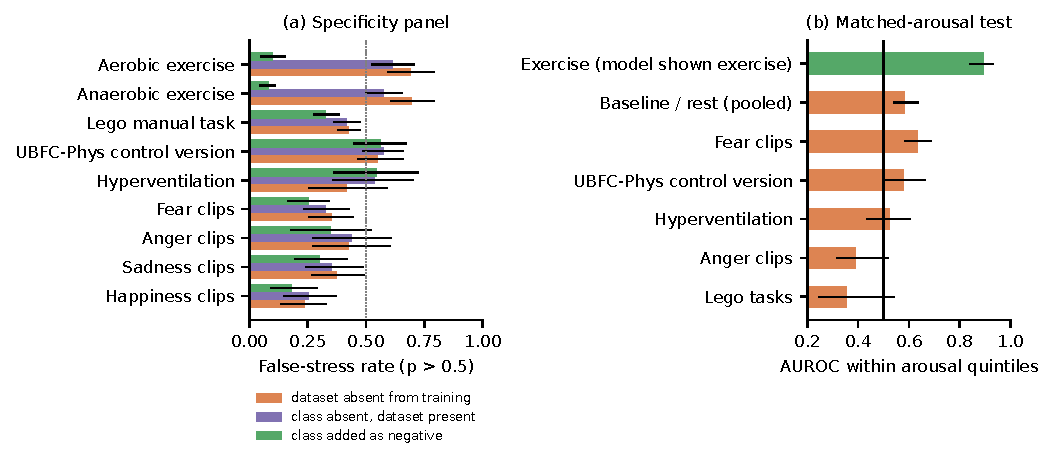
\includegraphics[width=\textwidth]{fig_panel.pdf}
\caption{(a) Specificity panel: false-stress rate of the HR/HRV/EDA detector on states absent from its task definition, under three training conditions, with subject-bootstrap 95\% CIs. (b) Matched-arousal test: within-bin AUROC of the stress score for stress versus each state (external model; for exercise, the model that has seen exercise). Only exercise, and fear clips once in training, remain separable at equal arousal.}
\label{fig:panel}
\end{figure*}

Fig.~\ref{fig:panel}(a) scores states that the LODO task never saw. A model without exercise calls 69--70\% of PhysioNet exercise windows stress, matching Aydo\u{g}an and Villagra Povina~\cite{aydogan2026}; training on all five datasets with exercise still excluded leaves 58--61\%, so the missing state, not the missing dataset, causes the alarms. Scoring these windows lowers external PhysioNet BA from 0.746 to 0.583 ($p_{\mathrm{holm}}=0.011$); adding exercise to the training negatives collapses the rate to 8--10\%. No other state behaves this way. The UBFC-Phys control group, performing the same speech and arithmetic without an evaluating panel, is called stress at 0.55--0.57 whether or not the model has seen it; hyperventilation stays at 0.42--0.55, Lego tasks fall only from 0.43 to 0.33, and emotion clips by 0.05--0.09. Stress recall is unchanged or higher when a state is added, so this is not a sensitivity trade-off.

\subsection{Matched-arousal test}
\begin{table}[!t]
\centering
\caption{Matched-Arousal Test: Within-Bin AUROC of the Stress Score}
\label{tab:matched}
\scriptsize
\begin{tabularx}{\columnwidth}{@{}Lrcccc@{}}
\toprule
Stress versus & $n$ & Pooled & Within-bin [CI] & $p_{\mathrm{holm}}$ & Disj. \\
\midrule
Lego manual task & 667 & 0.754 & 0.355 [0.24, 0.54] & 0.13 & 0.44 \\
UBFC-Phys, no evaluation & 80 & 0.587 & 0.577 [0.50, 0.67] & 0.41 & 0.52 \\
Hyperventilation & 53 & 0.551 & 0.523 [0.44, 0.61] & 0.62 & 0.52 \\
Anger clips & 33 & 0.643 & 0.390 [0.31, 0.52] & 0.41 & 0.41 \\
Fear clips & 394 & 0.716 & 0.633 [0.58, 0.69] & 0.004 & 0.65 \\
Baseline and rest & 3839 & 0.770 & 0.584 [0.54, 0.64] & 0.004 & 0.57 \\
\midrule
\multicolumn{6}{@{}l}{\emph{Probed state added to the training negatives}} \\
Exercise & 3763 & 0.947 & \textbf{0.892} [0.84, 0.93] & 0.003 & 0.88 \\
Fear clips & 394 & 0.804 & \textbf{0.779} [0.74, 0.82] & 0.003 & 0.78 \\
Lego manual task & 667 & 0.858 & 0.496 [0.44, 0.70] & 0.94 & 0.52 \\
UBFC-Phys, no evaluation & 80 & 0.583 & 0.568 [0.46, 0.67] & 0.64 & 0.50 \\
Hyperventilation & 53 & 0.568 & 0.560 [0.45, 0.67] & 0.64 & 0.54 \\
Anger clips & 33 & 0.699 & 0.431 [0.33, 0.62] & 0.64 & 0.52 \\
\bottomrule
\end{tabularx}
\par\vspace{2pt}\raggedright\scriptsize $n$: probe windows. CI: subject bootstrap; $p_{\mathrm{holm}}$: within-bin permutation test against 0.5, Holm-corrected per model. Disj.: index features and \texttt{eda\_mean} removed from the model.
\end{table}

At equal arousal the external detector does not separate stress from evaluated-versus-non-evaluated speech and arithmetic (within-bin AUROC 0.577), hyperventilation (0.523), Lego (0.355) or anger clips (0.390); none differs from chance after Holm correction (Table~\ref{tab:matched}), and adding the state to training does not change this ($p_{\mathrm{holm}}\ge0.64$). Exercise (0.892) and fear clips (0.779) become separable once in training; the exercise AUROC exceeds every non-separable pair (bootstrap lower bounds 0.18--0.36), and a heart-rate-only index gives 0.65 against 0.54 for an EDA-only index, so exercise is separated by its cardiac signature. Removing the index features from the model changes nothing (``Disj.''). With a heart-rate-only index and an EDA-only model, which approximates the iso-heart-rate test of Kwon et al., stress stays separable from rest (0.68, $p_{\mathrm{holm}}=0.0035$) but not from the UBFC-Phys control task (0.47) or hyperventilation (0.45). The two results agree: EDA separates stress from rest at equal heart rate, and neither channel separates stress from arousing non-stress tasks at equal heart rate and EDA. Two variant-specific exceptions (Lego with a heart-rate index, restricted to the 259 Lego windows with usable pulse; anger with an EDA index once in training, 0.74) do not change this.

\begin{table}[!t]
\centering
\caption{Arousal-Controlled Checks per Dataset (External Model, Stress vs All Non-Stress, AUROC [95\% CI])}
\label{tab:kit}
\scriptsize
\begin{tabularx}{\columnwidth}{@{}Lcccc@{}}
\toprule
Dataset & Index alone & Model $-$ index & Iso-HR & Residual \\
\midrule
WESAD & 0.952 & 0.016 [\m0.02, 0.07] & 0.957 & 0.63 [0.53, 0.71] \\
PhysioNet & 0.804 & 0.003 [\m0.06, 0.06] & 0.731 & 0.65 [0.56, 0.73] \\
Stress-Predict & 0.739 & \m0.031 [\m0.06, 0.00] & 0.674 & 0.59 [0.54, 0.63] \\
UBFC-Phys & 0.840 & 0.066 [0.00, 0.15] & 0.984 & 0.73 [0.63, 0.82] \\
Campanella & 0.948 & \m0.030 [\m0.08, 0.01] & 0.993 & 0.59 [0.46, 0.71] \\
\bottomrule
\end{tabularx}
\par\vspace{2pt}\raggedright\scriptsize Index: mean of per-subject z-scored HR and tonic EDA, no training. Iso-HR: within-subject 5-bpm HR bins, majority class subsampled, 7 seeds~\cite{kwon2026}. Residual: model logit after regressing it on the index within each dataset.
\end{table}

Table~\ref{tab:kit} asks how much of the detector is arousal. The untrained index ranks stress as well as the trained external model on every dataset (paired differences include zero on four datasets and touch it on UBFC-Phys) and explains 51--68\% of the variance of the model's logit. Kwon et al.'s iso-heart-rate test reproduces on all five datasets (0.67--0.99); against Lego it gives 0.69 where the heart-rate-and-EDA match gives 0.36, because heart-rate matching leaves the electrodermal part of arousal free. The residual still ranks stress above chance (0.59--0.73). At matched arousal the detector scores Lego (0.79 [0.70, 0.88]), anger (0.71), the UBFC-Phys control task (0.70) and hyperventilation (0.62) above rest, but not exercise (0.49) or fear (0.54): what it adds to arousal is shared by every active task, not specific to evaluation. The nulls are not proofs of equivalence: a synthetic positive control shows that the test detects within-bin AUROC of 0.60--0.64 and above for the four non-separable pairs, so a moderate evaluative signature is ruled out, a small one is not.

\subsection{Time in session and sensor warm-up}\label{sec:time}
\begin{figure*}[!t]
\centering
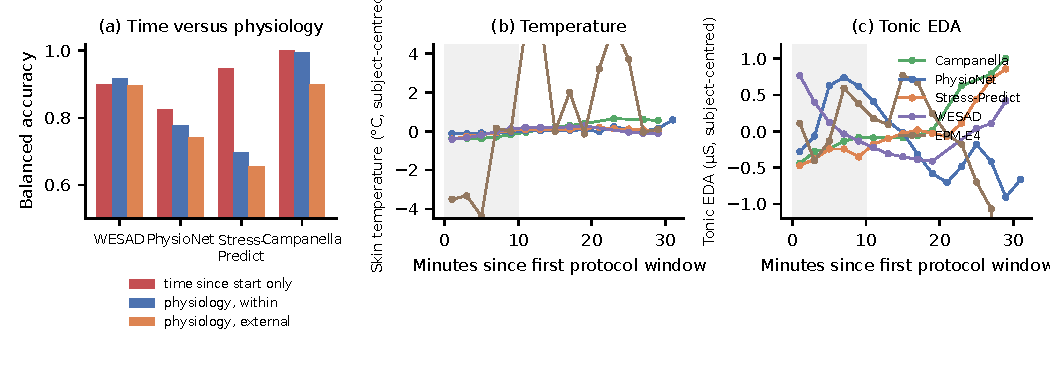
\includegraphics[width=\textwidth]{fig_time.pdf}
\caption{(a) Balanced accuracy of a classifier that sees only minutes since recording start, against the physiology model. (b), (c) Subject-centred skin temperature and tonic EDA against minutes since the first protocol window; the shaded band marks the first 10 min, in which 100\% of Campanella, 97\% of Stress-Predict and 68\% of PhysioNet baseline windows fall. WESAD's protocol clock starts 16--26 min after its recording.}
\label{fig:time}
\end{figure*}

Baseline is recorded first in every dataset. Minutes since recording start, used as the only feature, reach BA 0.83 on PhysioNet (physiology 0.78; better in 16 of 20 splits) and 0.95 on Stress-Predict (physiology 0.70; 20 of 20), tie on WESAD and are perfect on Campanella (Fig.~\ref{fig:time}a). A model given time exploits it within dataset (Stress-Predict 0.70 to 0.95) and collapses externally (0.66 to 0.56; WESAD 0.90 to 0.45). The physiology model survives position-matched negatives (changes of at most $-0.03$ within and $-0.04$ externally), so the LODO result does not ride on time; but the time-only classifier still reaches 0.88 on Stress-Predict after matching, so matching should accompany, not replace, a report of the time-only classifier. Time is informative because baseline coincides with sensor warm-up: measured from recording start, skin temperature rises at 0.02--0.08\,$^\circ$C/min and tonic EDA rises in the first 10 min on all four datasets with a continuous clock, and baseline falls inside that phase on Campanella (100\% of windows), Stress-Predict (97\%) and PhysioNet (68\% within 10 min, 90\% within 15). WESAD's baseline begins 17--49 min after the device is switched on, and it is the one dataset where time does not beat physiology. This quantifies the sequence effect described by Richer et al.~\cite{richer2024}.

\subsection{Error budget and stressor potency}
\begin{table}[!t]
\centering
\caption{Test-Side Error Budget: Shapley-Averaged BA Gain of Each Filter (HR/HRV/EDA)}
\label{tab:budget}
\scriptsize
\begin{tabularx}{\columnwidth}{@{}Lcccccc@{}}
\toprule
Dataset, model & All & F1 & F2 & F3 & F4 & Resid. \\
\midrule
PhysioNet, within & 0.776 & 0.003 & 0.007 & 0.020 & 0.020 & 0.175 \\
PhysioNet, external & 0.746 & 0.015 & 0.006 & 0.036 & 0.008 & 0.190 \\
Stress-Predict, within & 0.710 & 0.019 & 0.011 & 0.018 & 0.012 & 0.229 \\
Stress-Predict, external & 0.653 & 0.015 & \m0.015 & 0.012 & 0.005 & 0.329 \\
WESAD, external & 0.887 & 0 & 0.045 & 0 & 0.002 & 0.066 \\
\bottomrule
\end{tabularx}
\par\vspace{2pt}\raggedright\scriptsize F1: drop rest within 5 min of a stressor offset. F2: cardiac coverage $\ge$0.5. F3: drop the first 60 s of each stressor. F4: responders only (label-using, diagnostic).
\end{table}

Four test-side filters for recovery contamination, sensor loss, onset latency and non-response together buy 0.05--0.06 BA on PhysioNet and Stress-Predict (Table~\ref{tab:budget}); the residual error of 0.17--0.23 (0.33 external on Stress-Predict) is explained by none. A strict responder rule (1.0 baseline SD on both HR and tonic EDA) is the one term sensitive to its definition: it keeps 17 of 35 PhysioNet subjects and gains 0.094 [0.05, 0.15], but nothing on Stress-Predict. On WESAD the only sizeable term is the sensor; replacing wrist cardiac features with chest ECG raises BA from 0.916 to 0.956, so motion-robust wrist heart rate is worth at most about 0.04.

A dose--response test locates the rest (\texttt{stressor\_potency.py}). Over 182 subject-by-stressor units (123 subjects, 8 stressors), external recall rises with the subject's own arousal response to that stressor (index change from baseline; $\rho=0.56$ [0.43, 0.66]). Response alone explains 33\% of the variance in recall; dataset identity adds 0.10 [0.04, 0.21], while response adds 0.22 [0.13, 0.32] beyond dataset. The weakest stressor, Stress-Predict's Stroop, has both the smallest mean response (0.48 z) and the lowest recall (0.24). The ceiling is therefore set mainly, but not only, by how strongly each subject responds. Because the detector is close to an arousal index, this is expected; the informative result is that dataset identity explains little once response is known.

\subsection{Negative results}
On top of per-subject normalisation, unsupervised domain adaptation (correlation alignment, maximum mean discrepancy, adversarial networks) does not beat source-only training between WESAD and PhysioNet (0.54--0.70 both). Few-shot personalisation of a model trained on the other datasets, with each user's first $k=1$--5 windows per class and a 30-s gap, adds at most 0.02--0.04 BA, none significant; only random calibration windows give significant gains, as expected from leakage~\cite{tervonen2026,akkaya2026}. A per-user threshold hurts PhysioNet ($-0.08$). Self-rated stress does not predict which windows are missed (PhysioNet $\rho=0.02$ [$-0.30$, 0.31]); on WESAD the relation runs the other way ($\rho=-0.60$ [$-0.84$, $-0.08$], 15 subjects). Recall is not correlated across stressors within subjects, and is predicted by baseline physiology or pulse coverage in one of 16 tests.

\section{Discussion}
\emph{What wrist detectors detect.} A wrist device sees sympathetic arousal through a low-fidelity window. Once labels are protocol-anchored and features normalised per subject, the distributions of that arousal are similar across laboratory datasets, so a detector transfers at small cost and domain adaptation has nothing to align. What it has learned is arousal magnitude, which a two-feature index matches; a cardiac signature that sets exercise apart; and a residual shared by every active task. It has not learned evaluative threat: at equal arousal it cannot tell an evaluated speech from an unevaluated one, subtraction from Lego, or a stressor from hyperventilation. In the terms of psychophysiological inference~\cite{cacioppo2007}, laboratory protocols estimate P(signal $\mid$ stressor), whereas a deployed detector claims P(stress $\mid$ signal), and ``these conditional probabilities are equal only when the relationship [\ldots] is 1:1''. The panel and the matched test estimate the second direction and find the mapping many-to-one. The self-report and personalisation nulls follow: self-report is the wrong ruler for an arousal detector, and calibration cannot recover a response that did not occur.

\emph{Reporting norms.} We propose that a wearable stress detector be published with a specificity panel, its false-stress rate under exercise, speech without evaluation, cognitive load without threat and strong emotion, as an assay reports cross-reactivity; with a matched-arousal test and the untrained index as a baseline; with a settling period before baseline or time since donning as a covariate; with the time-only classifier reported whenever baseline precedes the stressor; and with exercise among the training negatives whenever the deployment includes movement.

\emph{Limitations.} Whole-session normalisation is transductive; the raw variant keeps the small cost, the causal one loses about 0.10 on short recordings. The hyperventilation and UBFC-Phys control cells are small, the UBFC-Phys contrast is between subjects, and effects below a within-bin AUROC of about 0.60 cannot be excluded. Wrist EDA agrees with palmar EDA at about $r=0.3$~\cite{milstein2020}, so an absent evaluative signature may be instrument failure. Responder filters use test labels and are diagnostic. All data are laboratory recordings from 132 subjects (plus 33 probe subjects). No public E4 dataset crosses speech with evaluation within subject or counterbalances order; such a study, with chest ECG and palmar EDA, is the decisive next step.

\section{Conclusion}
Across five public E4 datasets with audited labels, a wrist stress detector transfers to an unseen dataset at a cost of 0.015--0.05 BA, and an untrained index of heart rate and tonic EDA does as well. What transfers is autonomic arousal. The detector separates exercise once shown it, but at equal arousal it cannot separate evaluative stress from the same tasks without evaluation, from hyperventilation, manual work or anger clips. Protocol position predicts stress on datasets whose baselines coincide with sensor warm-up, and the within-dataset ceiling follows each subject's arousal response more than the pipeline. Progress is more likely to come from protocol design, contextual sensing and honest reporting than from classifiers.

\section*{Data and Code Availability}
The datasets are available from their original sources. The scripts that regenerate the audited labels and the 20 frozen subject splits, all analysis scripts and every result table cited here are at \url{https://github.com/ALVAROI12/smartwatch-stress-detection} (branch \texttt{jbhi-revision}).

\begin{thebibliography}{99}
\bibitem{prajod2024} P. Prajod, B. Mahesh, and E. Andr\'e, ``Stressor type matters!---Exploring factors influencing cross-dataset generalizability of physiological stress detection,'' in \emph{Proc. Int. Conf. Multimodal Interaction (ICMI)}, 2024, pp. 508--517, doi: 10.1145/3678957.3685741.
\bibitem{calzametre2026} M. Calza-Metre and L. Borz\`i, ``Machine learning-based automatic stress detection: Performance and generalization across datasets,'' \emph{Smart Health}, vol. 41, Art. no. 100693, 2026, doi: 10.1016/j.smhl.2026.100693.
\bibitem{xiao2025} Y. Xiao, H. Sharma, S. Kaur, D. Bergen-Cico, and A. Salekin, ``Human heterogeneity invariant stress sensing,'' \emph{Proc. ACM Interact. Mob. Wearable Ubiquitous Technol.}, vol. 9, no. 3, Art. no. 3749465, pp. 1--42, 2025, doi: 10.1145/3749465.
\bibitem{mishra2020} V. Mishra, S. Sen, G. Chen, T. Hao, J. Rogers, C.-H. Chen, and D. Kotz, ``Evaluating the reproducibility of physiological stress detection models,'' \emph{Proc. ACM Interact. Mob. Wearable Ubiquitous Technol.}, vol. 4, no. 4, Art. no. 147, 2020, doi: 10.1145/3432220.
\bibitem{zhou2023} E. Zhou, M. Soleymani, and M. J. Matari\'c, ``Investigating the generalizability of physiological characteristics of anxiety,'' in \emph{Proc. IEEE Int. Conf. Bioinformatics Biomed. (BIBM)}, 2023, pp. 4848--4855, doi: 10.1109/BIBM58861.2023.10385292.
\bibitem{kwon2026} N. Kwon, S. Yoon, J. Hur, and H. S. Kang, ``When wellness stress detection enters healthcare workflows: An iso-heart-rate, cross-corpus evaluation of wrist wearables,'' \emph{Healthcare}, vol. 14, no. 15, Art. no. 2434, 2026, doi: 10.3390/healthcare14152434.
\bibitem{schreiber2026} P. Schreiber and M. Maleshkova, ``AutoStress benchmark: Evaluating factors that influence cross dataset generalizabilty in stress recognition,'' in \emph{Proc. IEEE Conf. Artif. Intell. (CAI)}, 2026, pp. 1335--1341, doi: 10.1109/CAI68641.2026.11536323.
\bibitem{singh2026feel} P. Singh, A. Gupta, S. Jalan, M. Kumar, and P. Singh, ``FEEL: Quantifying heterogeneity in physiological signals for generalizable emotion recognition,'' arXiv preprint arXiv:2604.05926, 2026, doi: 10.48550/arXiv.2604.05926.
\bibitem{aydogan2026} Y. Aydo\u{g}an and F. Villagra Povina, ``Stress or arousal? Exercise confounding in wearable stress detection,'' \emph{Med. Eng. Phys.}, vol. 147, Art. no. 095021, 2026, doi: 10.1088/1873-4030/aea41e.
\bibitem{richer2024} R. Richer \emph{et al.}, ``Machine learning-based detection of acute psychosocial stress from body posture and movements,'' \emph{Sci. Rep.}, vol. 14, Art. no. 8251, 2024, doi: 10.1038/s41598-024-59043-1.
\bibitem{tognotti2026} A. Tognotti, C. F. Otesteanu, L. Anceschi, and C. Menon, ``Baseline normalization choices inflate classification performance in wearable health monitoring: Quantification and mitigation strategies,'' \emph{Front. Digit. Health}, vol. 8, Art. no. 1827279, 2026, doi: 10.3389/fdgth.2026.1827279.
\bibitem{saeb2017} S. Saeb, L. Lonini, A. Jayaraman, D. C. Mohr, and K. P. Kording, ``The need to approximate the use-case in clinical machine learning,'' \emph{GigaScience}, vol. 6, no. 5, 2017, doi: 10.1093/gigascience/gix019.
\bibitem{bahameish2024} M. Bahameish, T. Stockman, and J. Requena Carri\'on, ``Strategies for reliable stress recognition: A machine learning approach using heart rate variability features,'' \emph{Sensors}, vol. 24, no. 10, Art. no. 3210, 2024, doi: 10.3390/s24103210.
\bibitem{stewart2020} C. L. Stewart, A. Folarin, and R. Dobson, ``Personalized acute stress classification from physiological signals with neural processes,'' arXiv preprint arXiv:2002.04176, 2020, doi: 10.48550/arXiv.2002.04176.
\bibitem{han2024} Y. Han, P. Zhang, M. Park, and U. Lee, ``Systematic evaluation of personalized deep learning models for affect recognition,'' \emph{Proc. ACM Interact. Mob. Wearable Ubiquitous Technol.}, vol. 8, no. 4, Art. no. 206, pp. 1--35, 2024, doi: 10.1145/3699724.
\bibitem{tervonen2026} J. Tervonen, E. Amparore, M. Botta, J. N\"arv\"ainen, K. Pettersson, and J. M\"antyj\"arvi, ``Data-constrained personalization of cognitive state detection with feature-based and foundation models,'' \emph{User Model. User-Adapt. Interact.}, 2026, doi: 10.1007/s11257-026-09444-w.
\bibitem{akkaya2026} A. Akkaya, ``Calibration, not architecture, limits cross-subject wearable stress detection: A multi-dataset, decision-focused evaluation with label-efficient recalibration,'' \emph{BMC Med. Inform. Decis. Mak.}, 2026, doi: 10.1186/s12911-026-03842-1 (abstract only).
\bibitem{milstein2020} N. Milstein and I. Gordon, ``Validating measures of electrodermal activity and heart rate variability derived from the Empatica E4 utilized in research settings that involve interactive dyadic states,'' \emph{Front. Behav. Neurosci.}, vol. 14, Art. no. 148, 2020, doi: 10.3389/fnbeh.2020.00148.
\bibitem{watanabe2025} Y. Watanabe, N. Yamane, A. Sathyanarayana, V. Mishra, and M. S. Goodwin, ``Beyond motion artifacts: Optimizing PPG preprocessing for accurate pulse rate variability estimation,'' in \emph{Companion Proc. ACM Int. Joint Conf. Pervasive Ubiquitous Comput. (UbiComp Companion)}, 2025, pp. 1176--1182, doi: 10.1145/3714394.3756241.
\bibitem{sosa2026} S. Sosa, A. K. Fontecchio, E. G. Chrysikou, and J. S. Atchison, ``Beyond EDA: A systematic review of multimodal sympathetic nervous system arousal classification for stress detection,'' \emph{Sensors}, vol. 26, no. 5, Art. no. 1584, 2026, doi: 10.3390/s26051584.
\bibitem{schmidt2018wesad} P. Schmidt, A. Reiss, R. D\"urichen, C. Marberger, and K. Van Laerhoven, ``Introducing WESAD, a multimodal dataset for wearable stress and affect detection,'' in \emph{Proc. Int. Conf. Multimodal Interaction (ICMI)}, 2018, doi: 10.1145/3242969.3242985.
\bibitem{hongn2025data} A. Hongn, F. Bosch, L. E. Prado, J. M. Ferr\'andez, and M. P. Bonomini, ``Wearable physiological signals under acute stress and exercise conditions,'' \emph{Sci. Data}, vol. 12, Art. no. 520, 2025, doi: 10.1038/s41597-025-04845-9.
\bibitem{iqbal2022} T. Iqbal \emph{et al.}, ``Stress monitoring using wearable sensors: A pilot study and Stress-Predict dataset,'' \emph{Sensors}, vol. 22, no. 21, Art. no. 8135, 2022, doi: 10.3390/s22218135.
\bibitem{meziati2023} R. Meziati Sabour, Y. Benezeth, P. De Oliveira, J. Chapp\'e, and F. Yang, ``UBFC-Phys: A multimodal database for psychophysiological studies of social stress,'' \emph{IEEE Trans. Affect. Comput.}, vol. 14, no. 1, pp. 622--636, 2023, doi: 10.1109/TAFFC.2021.3056960.
\bibitem{campanella2024} S. Campanella, A. Altaleb, A. Belli, P. Pierleoni, and L. Palma, ``PPG and EDA dataset collected with Empatica E4 for stress assessment,'' \emph{Data Brief}, vol. 53, Art. no. 110102, 2024, doi: 10.1016/j.dib.2024.110102.
\bibitem{garcia2020epm} F. M. Garcia-Moreno and M. Badenes-Sastre, ``EmoPulse Moments E4 dataset (EPM-E4): An exhaustive collection of emotion-related data from Empatica E4 wearable,'' Zenodo, 2020, doi: 10.5281/zenodo.8431638.
\bibitem{cacioppo2007} J. T. Cacioppo, L. G. Tassinary, and G. G. Berntson, ``Psychophysiological science: Interdisciplinary approaches to classic questions about the mind,'' in \emph{Handbook of Psychophysiology}, 3rd ed., J. T. Cacioppo, L. G. Tassinary, and G. G. Berntson, Eds. Cambridge, U.K.: Cambridge Univ. Press, 2007, ch. 1.
\bibitem{nadeau2003} C. Nadeau and Y. Bengio, ``Inference for the generalization error,'' \emph{Mach. Learn.}, vol. 52, no. 3, pp. 239--281, 2003, doi: 10.1023/A:1024068626366.
\end{thebibliography}

\end{document}
